% TBD by Wolfgang
\subsection{Style Viewers} 
\label{sec:viewers}
As we have shown earlier, the style views are the essence of the creative process so it's worth looking at this in its raw form. That's why we included some style viewers into the project to apply to this task. In this section we introduce them.

\subsubsection{Text Based viewer}
\label{sec:viewers.text}
As discussed earlier the styles are saved in a JSON file. Even though this format is made to be readable by humans we thought of a more pleasant way to view the style while developing. So we gave the style objects a print method. This method will print the style onto the current output of your python session, as can be seen in the figure below:
\begin{figure}[ht]
\centering
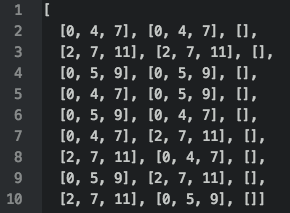
\includegraphics[scale=1]{Chapters/pic/text_print.png}
\caption{A sample chord printed with the print method}
\end{figure}

This figure shows the dummy style. The viewer orders all the style sequences according to their likelihood, starting with the most likely. It also translates our numeric representation into a tonal representation for a given key (default key is C major).

That way we can easily see how the style will look like and if after applying the creative module an odd thing happened to the style, that would be harder to spot after the actual harmonizer. 

\subsubsection{MusicXML Creator}
\label{sec:viewers.musicxml}
Also faster and more visual would be to translate the style into a MusicXML file and view it with your favorite MusicXML viewer. We used MuseScore for that purpose. 

\begin{figure}[ht]
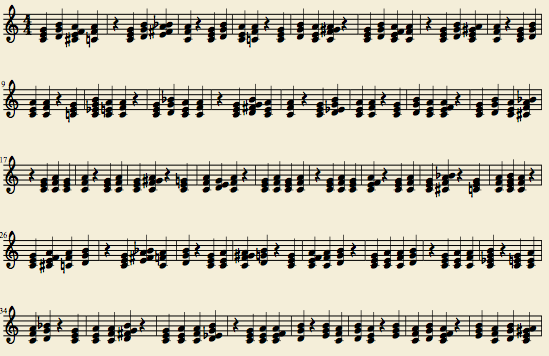
\includegraphics[scale=.5]{Chapters/pic/xml_print.png}
\caption{MusicXML of a sample style viewed with the MuseScore program}
\end{figure}

As seen in the figure above we used the write MusicXML method of the visualizer. It does the same thing as the print method, that it orders the chord sequences starting with the most likely. But instead of printing it to the output it creates a MusicXML file. For convenience we defined a bunch of default values, namely the key is C major, the duration of a tone is quarter pitch, as well as we use a four quarters rhythm. After every sequence we inserted a quarter break to indicate the end of a harmonization sequence.

With this visualization you have the major advantage that now you have standardized data structure and you are able to process them further. But mainly you want to view it in a score notation or listen to your creation.

\subsubsection{Extempore}
\label{sec:viewers.extempore}

Finally, the best way to get an intuitive impression of a style is to listen to it.
This is the purpose of the Extempore (cf. \ref{sec:tools.extempore}) based style ``viewer'', which takes the chord progressions from a style description and plays a continuous stream of chords based on these progressions.
The next progression is determined by selecting all progressions that start with the last chord of the current progression and choosing randomly with a bias according to the progressions' weights.
If no matching progression is available, the system chooses from all progressions.

The playback is done by a simple simulation of a jazz trio, i.e., a bass, a drum set, and a piano.
Each chord is played for one bar (four beats) and all instruments are based on prerecorded samples. The drums play a fixed simple swing rhythm that repeats every two beats.

The bass simulates a walking bass and plays either one note per beat or in some cases randomly two swing eights per beat.
The next note is chosen based on the previous note: within a range of two octaves around the previous note, each note that belongs to the current chord is given a weight which decreases with increasing distance to the previous note.
Upper and lower limits are used to restrict the notes to an absolute range.
The next note is then picked randomly with respect to the weights.

The piano takes the current chord and picks four random notes that belong to the chord from a given range.
This set of notes is then repeatedly played as a chord according to a randomly generated rhythm.
The rhythm is determined by a coin flip for each eighth of a bar whether a note should start on it and an additional coin flip for each note whether it should be short (i.e., 1/3 beat = a short swing eighth) or long (i.e., until the next note starts).

In its current form, this is not only a very subjective and intuitive approach to the evaluation of a style but is also biased by being fitted to simulating a typical style of jazz music.
It might, however, be adapted to be more neutral.